\documentclass[11pt, a4paper]{article}
\usepackage[utf8]{inputenc}
\usepackage[top=0.1in, left=0.5in, bottom=0.5in, right=0.5in]{geometry} 
%\addtolength{\topmargin}{-0.4in}
%\usepackage{amsmath} %Only load this if you are using math/equations.
\usepackage{graphicx} %Only need to call this if inserting images.
\usepackage{caption} %Only need to call this if inserting captions.
\usepackage{float} %Allows the use of the [H] specifier.
\usepackage{setspace}
\usepackage{blindtext}

%\pagenumbering{arabic}
%\thispagestyle{empty}

%\usepackage{fontspec} %%in order for this font stuff to work, you must compile using xelatex+makeindex+bibtex (or at minimum xelatex)
%\setmainfont[Mapping=tex-text-ms]{Essays1743}

\usepackage{fancyhdr}

\pagestyle{fancy}
\fancyhf{}
 \renewcommand{\headrulewidth}{0pt} 
\rhead{}
\lhead{}
\cfoot{References available upon request.}


\usepackage{tikz}
\usetikzlibrary{shapes.misc, positioning}

%https://tex.stackexchange.com/questions/22406/how-to-make-a-textbox-with-this-tikz-code
\xdefinecolor{mycolor}{RGB}{62,96,111} % Neutral Blue
\colorlet{bancolor}{mycolor}

\def\bancolor{mycolor}
\newenvironment{mybox}[3][]{%
    \begin{tikzpicture}[#1]%
        \def\myboxname{#3}%
        \node [draw,inner sep=1.5ex,text width=#2]% good options: minimum height, minimum width
            (BOXCONTENT) \bgroup\rule{0pt}{3ex}\ignorespaces
}{%
        \egroup;
        \node [right,inner xsep=1em,fill=bancolor!75,outer sep=0pt,text height=2ex,text depth=.5ex] (BOXNAME) 
            at ([shift={(-1em,0pt)}]BOXCONTENT.north west) {\myboxname};
%        \fill[bancolor] (BOXNAME.north east) -- +(-1em,1em) -- +(-1em,0) -- cycle;
        \fill[bancolor] (BOXNAME.south west) -- +(1em,-1em) -- +(1em,0) -- cycle;
    \end{tikzpicture}
}




\newcommand{\comment}[1]{}

\usepackage{color}
\definecolor{silver}{RGB}{35,43,43}
\pagecolor{silver}
\color{white}

\xdefinecolor{mycolor2}{RGB}{255, 160, 0}
\colorlet{orange1}{mycolor2}
%\definecolor{orange1}{RGB}{255, 160, 0} 
\usepackage[colorlinks,citecolor=blue,linkcolor=blue,urlcolor=orange1]{hyperref} %Allows for the embedding of urls. 
\hypersetup{pdflinkmargin=0.8pc}


%fonts
\usepackage{fontspec}
%\setmainfont{Gotham Book}
\setmainfont{Gotham Book}[
  Path = ./Gotham-Font/ ,
  Extension       =  .ttf ,
  UprightFont     =  GothamBook    ,
  ItalicFont      =  GothamBookItalic ,
  BoldFont        =  GothamBold    , 
  BoldItalicFont  =  GothamBoldItalic ,
]










\begin{document}

\noindent
\begin{minipage}{0.6\textwidth}
\noindent {\fontsize{32}{10}\selectfont \textbf{Jonah Edmundson}}
\normalsize
\par
\vspace{0.2pc}
\hspace{18.4pc}
\textit{Data Scientist}
\end{minipage}\hfill
\hspace{2pc}\begin{minipage}{0.4\textwidth}
\begin{flushright}
\footnotesize
\noindent Email: \par
\noindent \href{mailto:jonahedmundson@gmail.com}{\url{jonahedmundson@gmail.com}}
\par
%\vspace{0.75pc}
\par
\noindent Website: \par
\noindent \href{www.jonahedmundson.xyz}{\url{www.jonahedmundson.xyz}}
\par
%\vspace{0.75pc}
\par
\noindent LinkedIn: \par
\noindent \href{https://www.linkedin.com/in/jonah-edmundson-109151258/}{\url{linkedin.com/in/jonah-edmundson-109151258/}}
\par
\noindent GitHub: \par
\noindent \href{https://github.com/jonahedmundson}{\url{github.com/jonahedmundson}}

%\url{https://github.com/jonahedmundson}
\end{flushright}
\end{minipage}



\normalsize
\noindent

\begin{figure}[H]
\begin{minipage}[t]{0.7\textwidth}
\noindent
\vspace{0pt}

\par

\vspace{1pc}

Hello! 
\par
I am a graduating data science student looking to break into the tech industry. I hope that my resume properly communicates my enthusiasm for this exciting field. \\

\vspace{1pc}

\comment{
\begin{mybox}{\textwidth}{Education}
    This is the longer content \\
    This is the longer content \\
    This is the longer content \\
    This is the longer content \\
    This is the longer content
\end{mybox}	
}


\textbf{\large{EDUCATION}}
\par\noindent\rule{\textwidth}{1.0pt}
\par
\vspace{0.5pc}

%\begin{flushleft}


\noindent\textit{Master's of Data Science} \\
\hspace{1pc} University of British Columbia Okanagan, Kelowna, BC \\
\hspace{1pc} Expected Graduation: Summer 2023 \\

\vspace{0.5pc}

\noindent\textit{Bachelor of Science}, 2022 \hfill GPA: 4.00 \\
\hspace{1pc} The King’s University, Edmonton, AB \\
\hspace{1pc} General Biology \\
\hspace{1pc} Minor in Philosophy

%\end{flushleft}

\par

\phantom{3pt} \\

\par

\textbf{\large{PROJECTS}} \hfill (clickable)
\par\noindent\rule{\textwidth}{1.0pt}
\par
\vspace{0.5pc}
%sideproject
%497
%dashboard
%pyquizlet?

\textit{\href{https://jonahedmundson.github.io/kelowna_weathercrash/}{Kelowna Weather-Crash} \hfill 2023} \\
A statistical investigation into the relationship between local weather trends and vehicle accidents in the city of Kelowna. 

\vspace{1.5pc}

\textit{\href{https://jonahedmundson.github.io/VGsalesDashboard_R/}{Video Games Dashboard} \hfill 2023} \\
A dashboard for video game sales using ggplot2 and R Dash. 

\vspace{1.5pc}

\textit{\href{https://www.jonahedmundson.xyz/edmundson\_finalsubmission.pdf}{BIOL497 Senior Thesis} \hfill 2022} \\ 
Analyzing the flow of substance misuse patients through the emergency department using a multi-state modelling approach.

\vspace{1.5pc}

\textit{\href{https://github.com/jonahedmundson/py\_quizlet\_cram}{Py Quizlet Kahoot} \hfill 2022} \\
A package for taking Quizlet and Kahoot quizzes in Python. Quizzes are webscraped in real time.




\par

\phantom{3pt} \\

\par

\textbf{\large{VOLUNTEERING}}
\par\noindent\rule{\textwidth}{1.0pt}
\par
\vspace{0.5pc}

\textit{The King’s Ambassadors \hfill 2018 - 2022}
\par
A volunteer group designed to represent the university and help with school-related events.

\vspace{1.5pc}

\textit{Kelowna Gospel Mission \hfill 2022 - Current}
\par
Helping prepare and serve food. Weekly. 








\end{minipage}\hfill
\hspace{2pc}\begin{minipage}[t]{0.3\textwidth}
\vspace{0pt}
\noindent 

\vspace{5pc}

\begin{tikzpicture}

	%moves whole pic slightly right
	%\node [] (Z) at (-2.5,0){};

	\node [draw, rounded rectangle] (title) at (0.2, 0){\LARGE Timeline}; 

%vertical line
	\coordinate [] (A) at (0,-11.5){};
	\coordinate [label={[align=right, label distance=-2cm]00:\textit{Summer}\\\textit{2023}}] (B) at (0,-10.5){};
	\coordinate [] (C) at (0,-9.5){};
	\coordinate [label={[align=right, label distance=-1.5cm]00:\textit{2023}}] (D) at (0,-8.5){};
	\coordinate [] (E) at (0,-1){};
	\coordinate [label={[align=right, label distance=-1.5cm]00:\textit{2022}}] (F) at (0,-6.5){};
	\coordinate [] (G) at (0,-5.5){};
	\coordinate [] (H) at (0,-4.5){};
    \coordinate [] (I) at (0,-3.5) {};
    \coordinate [label={[align=right, label distance=-1.4cm]00:\textit{2018}}] (J) at (0,-2.5) {};
    \coordinate [] (K) at (0,-1.5) {};
    
    \draw [white, very thick,<->,>=stealth] (A) -- (K);
    \filldraw[color=white, very thick](B) circle (0.1);
    \filldraw[color=white, very thick](J) circle (0.1);
    %\filldraw[color=white, very thick](H) circle (0.1);
    %\filldraw[color=white, very thick](K) circle (0.1);
    \filldraw[color=white, very thick](F) circle (0.1);
    \filldraw[color=white, very thick](D) circle (0.1);
    
%aux lines
    \coordinate [label={[align=left, label distance=0.2cm]00:High School\\Graduation}] (AF) at (0.15,-1.85){};
    %
    \coordinate [] (AA) at (0.3,-2.5){};
    \coordinate [] (AB) at (0.5,-2.5){};
    \coordinate [] (AC) at (0.5,-4.5){};
    \coordinate [] (AD) at (0.3,-6.4){};
    \coordinate [] (AE) at (0.5,-6.4){};
    \coordinate [label={[align=left, label distance=0.2cm]00:BSc\\Biology}] (AF) at (0.7,-4.5){};
	\draw [white, thick] (AA) -- (AB);
	\draw [white, thick] (AB) -- (AE);
	\draw [white, thick] (AD) -- (AE);
	\draw [white, thick] (AC) -- (AF);
	%
	\coordinate [] (AG) at (0.3,-6.6){};
    \coordinate [] (AH) at (0.5,-6.6){};
    \coordinate [] (AI) at (0.5,-7.5){};
    \coordinate [] (AJ) at (0.3,-8.5){};
    \coordinate [] (AK) at (0.5,-8.5){};
    \coordinate [label={[align=left, label distance=0.2cm]00:Master's of\\Data Science}] (AL) at (0.7,-7.5){};
	\draw [white, thick] (AG) -- (AH);
	\draw [white, thick] (AH) -- (AK);
	\draw [white, thick] (AJ) -- (AK);
	\draw [white, thick] (AI) -- (AL);
	%
	\coordinate [label={[align=center, label distance=0.2cm]00:\large\textbf{Working}\\\large\textbf{with you!}}] (AX) at (0.2,-10.5){};
	

\end{tikzpicture}

\vspace{2pc}


\begin{tikzpicture}

	%moves whole pic slightly right
	%\node [] (Z) at (-2.5,0){};
	\node [] (Z) at (0,0){};

	\node [draw, rounded rectangle] (title) at (2.2, 0){\LARGE Skills}; 
	
\end{tikzpicture}


\begin{center}
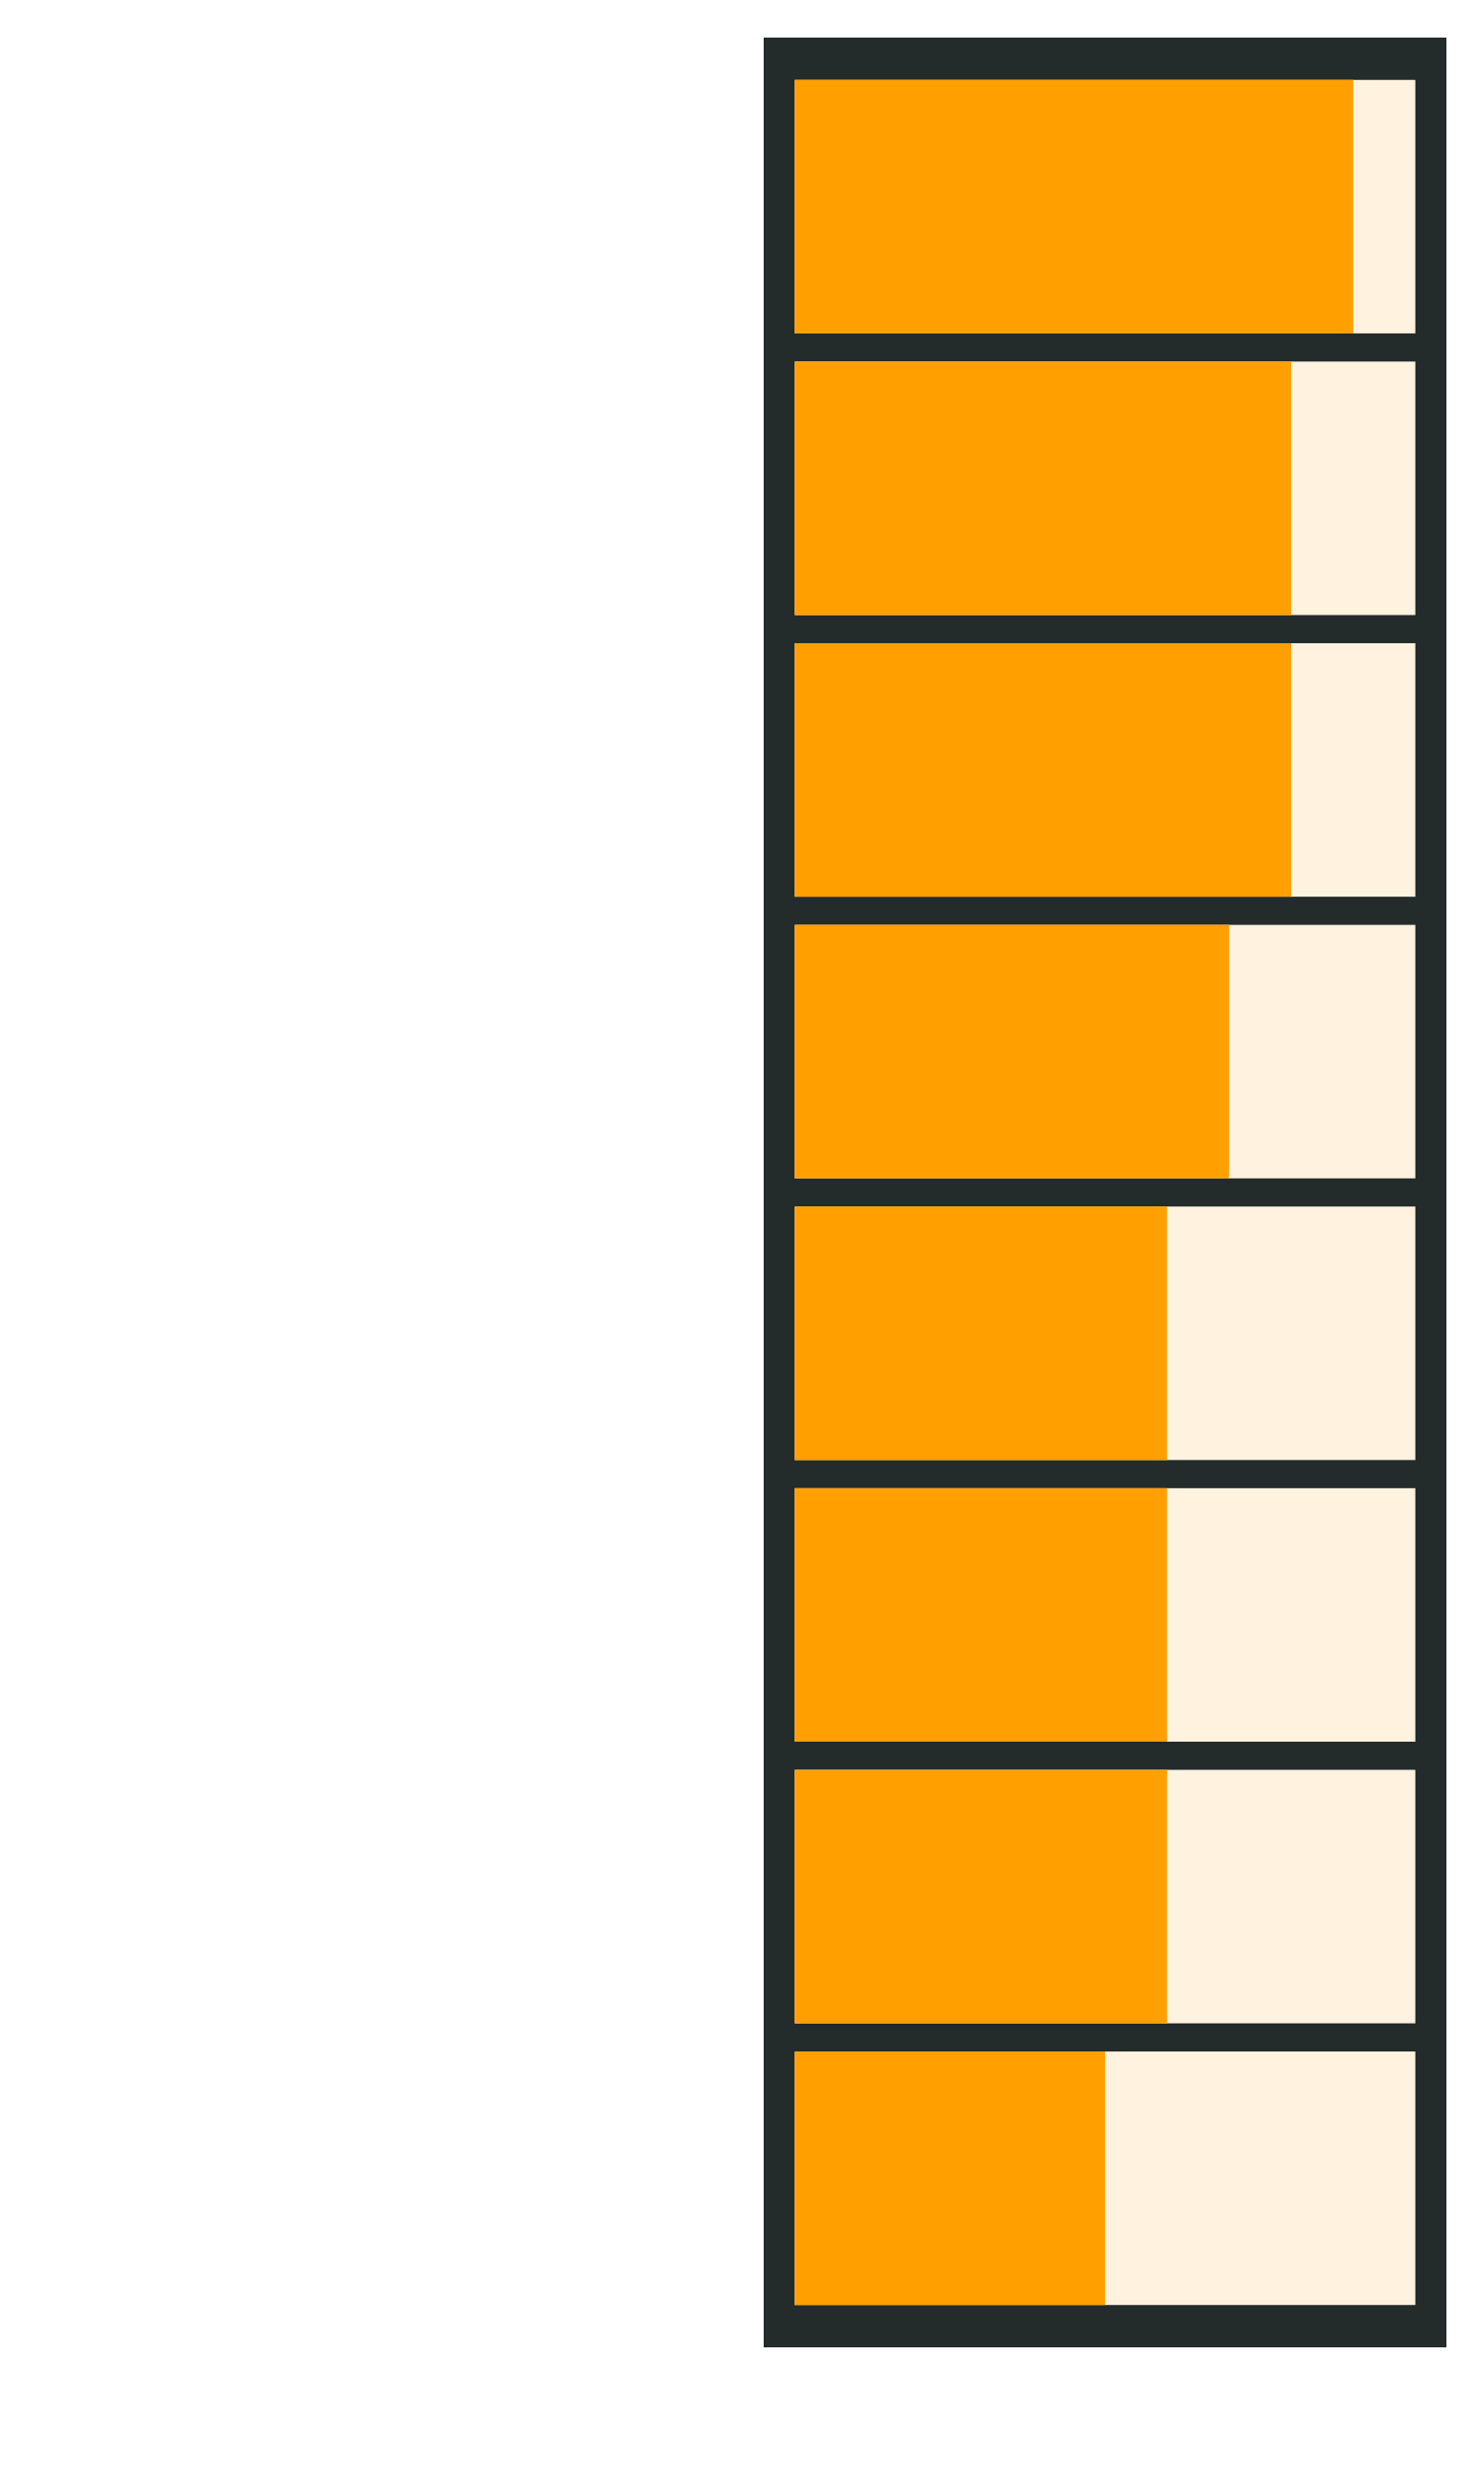
\includegraphics[width=0.9\textwidth]{./figures/skill_figure.png}
\end{center}


\end{minipage} 

\end{figure}


\comment{
\begin{figure}[H]
\begin{minipage}{0.9\textwidth}




\par

\phantom{0pt} \\

\par

\comment{
\begin{mybox}{\textwidth}{Awards}
    This is the longer content \\
    This is the longer content \\
    This is the longer content \\
    This is the longer content \\
    This is the longer content
\end{mybox}	
}










\end{minipage}
\end{figure}
} %end of long comment

\end{document}
